%%%%%%%%%%%%%%%%%%%%%%%%%%%%%%%%%%%%%%%%%
% Maxime FELICI
% LaTex Template
% Version 1.0 (09/09/17)
%%%%%%%%%%%%%%%%%%%%%%%%%%%%%%%%%%%%%%%%%



%----------------------------------------------------------------------------------------
%	PACKAGES AND DOCUMENT CONFIGURATIONS
%----------------------------------------------------------------------------------------
\documentclass{article}

\usepackage[utf8]{inputenc}
\usepackage[T1]{fontenc}
\usepackage[francais]{babel}
\usepackage[margin=3cm]{geometry}
\usepackage{verbatim}
\usepackage{moreverb}
\usepackage{listings}
\usepackage{graphicx}
\usepackage{calc}
\usepackage{fancyhdr}
\usepackage{textcomp}
\usepackage{amsmath,amsfonts,amssymb}
\usepackage{minted}
\usepackage{tcolorbox}
\usepackage{etoolbox}
\BeforeBeginEnvironment{minted}%
     {\begin{tcolorbox}}%
\AfterEndEnvironment{minted}
   {\end{tcolorbox}}%
\pagestyle{fancy}


%----------------------------------------------------------------------------------------
%	DOCUMENT INFORMATION
%----------------------------------------------------------------------------------------
\fancyhead[C]{CS441 - Génie Logiciel}
\fancyhead[L]{P2019}
\fancyhead[R]{\thedate}

\title{Mini-projet de développement d'une application de gestion de
tirages photos numériques}
\date{\today}

\makeatletter
\let\thetitle\@title
\let\theauthor\@author
\let\thedate\@date
\makeatother

\begin{document}
\begin{titlepage}
	\centering
    \vspace*{0.5 cm}
    
\includegraphics[scale = 0.75]{logo}\\[1.0 cm]	% University Logo
    \textsc{\LARGE Grenoble INP - Esisar}\\[2.0 cm]	% University Name
    	{\large \thedate}\\[0.3 cm]
	\textsc{\Large CS441}\\[0.3 cm]				% Course Code
	\textsc{\large Génie Logiciel}\\[0.3 cm]				% Course Name
  \vspace{1\baselineskip}
  \vspace{1\baselineskip}
  \vspace{1\baselineskip}
	\rule{\linewidth}{0.2 mm} \\[0.4 cm]
	{ \huge \bfseries \thetitle}\\
	\rule{\linewidth}{0.2 mm} \\[1.5 cm]
\vspace{1\baselineskip}
\vspace{1\baselineskip}
\vspace{1\baselineskip}
	\begin{minipage}{0.4\textwidth}
		\begin{flushleft} \large
			\emph{Auteurs : }\\
      Mathieu PLAINEMAISON \\
      Maxime FELICI \\
      Pauline MALOSSE \\
      Rémi POLETTI \\
      Anis BEN MAHMOUD \\
      Soraya AFELLAD \\
			\end{flushleft}
			\end{minipage}~
      \begin{minipage}{0.4\textwidth}
			\begin{flushright} \large
		\end{flushright}
	\end{minipage}\\[2 cm]



	\vfill

\end{titlepage}


\tableofcontents
\newpage
%DEBUT DU DOCUMENT
%------------------------------
\begin{flushleft}

%------------------------------
\section{Introduction}
L'objectif de ce projet est de mettre en oeuvre les techniques de Génie
Logiciel acquises en cours et en TD :
\vspace{1\baselineskip}
\begin{itemize}
  \item Travail en équipe
  \item Mise en place d'un cycle de vie, gestion des différents acteurs,
  gestion d'un planning, analyse des risques
  \item Rédaction de la documentation adaptée
  \item Modélisation de l'application
  \item Développement de l'application
  \item Tests des différentes fonctionnalités de l'application
\end{itemize}
\vspace{1\baselineskip}
Il faudra pour cela concevoir une application de gestion de tirages photos
numériques. Celle-ci utilisera la base de données Oracle 11i déployée à
l'Esisar, ainsi que le driver JDBC pour l'interroger. L'application doit
permettre à un client de se connecter, d'ajouter des photos, de créer et
supprimer des albums, de consulter la liste des commandes.



\section{Les acteurs du projet}
Dans le développement de cette application, il y a eu plusieurs acteurs : \\
\vspace{1\baselineskip}
\begin{itemize}
  \item \textbf{La maîtrise d'ouvrage} : Entreprise ou service "client".
  Il s'agit ici de la société de tirage de photos numérique sur l'internet
  \textbf{Esyphoto}.
  \item \textbf{La maîtrise d'oeuvre} : Entreprise ou service ayant pris
  l'engagement de réaliser le projet pour la maîtrise d'ouvrage. Il s'agit
  ici, pour la simulation, de l'Esisar.
  \item \textbf{La maîtrise d'oeuvre déléguée (ou chef de projet)} : C'est
  la personne en charge par la maîtrise d'oeuvre de mener à bien le projet.
  Dans notre cas, il s'agit
  de Mathieu PLAINEMAISON.
  \item \textbf{L'équipe de projet} : Elle est composée du reste des membres
  de l'équipe 2, à savoir Maxime FELICI, Pauline MALOSSE, Anis BEN MAHMOUD,
  Rémi POLETTI et Soraya AFELLAD.
\end{itemize}
\vspace{1\baselineskip}


\section{Cycle de vie choisi}

Nous avons décidé pour ce projet de suivre un cycle de vie en V :\\
\vspace{1\baselineskip}
\vspace{1\baselineskip}
\begin{minipage}{0.55\linewidth}
  \begin{center}
    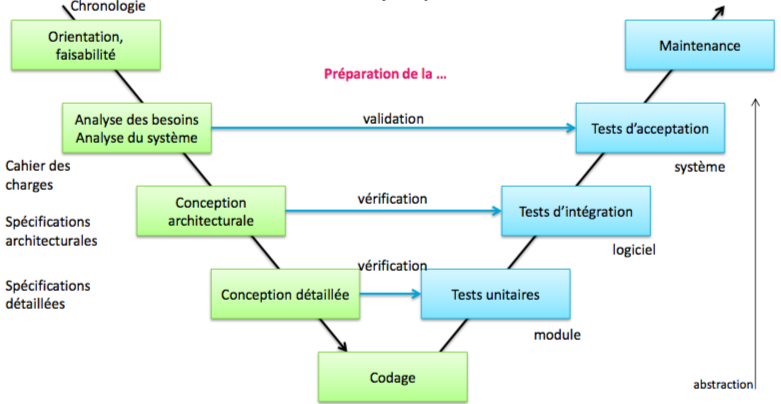
\includegraphics[scale=0.3]{fig5}
  \end{center}
\end{minipage}\hfill
\begin{minipage}{0.4\linewidth}
L'avantage de cette méthode est qu'elle est simple à comprendre pour
l'ensemble de l'équipe. Elle impose cependant une organisation stricte,
une validation et des tests à chaque étape et de la documentation.\\
Les deux premières étapes (Orientation, faisabilité et Analyse des
besoins/Analyse du système) ont déjà été faites dans le sujet.
\end{minipage}


\newpage

\section{Analyse des risques}

\begin{figure}[h]
  \begin{center}
    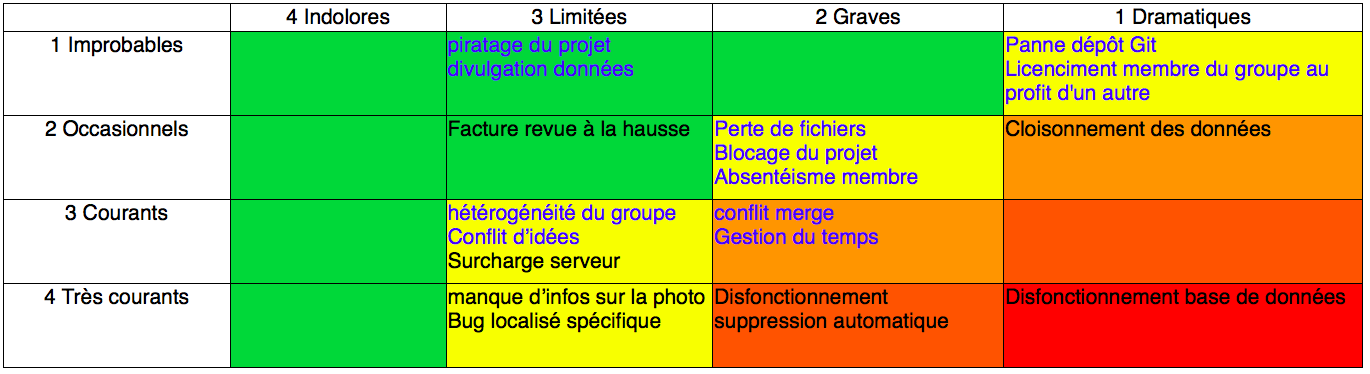
\includegraphics[scale=0.3]{fig3} % Include the image placeholder.png
    \caption{Tableau d'analyse des risques}
  \end{center}
\end{figure}

Lors de la première séance de projet, nous avons mit au point un tableau
d'analyse des risques. Un risque a été analysé comme "improbable" mais
"catastrophique". Il s'agit du licenciment d'un membre du groupe au profit
d'un autre. Ce licenciment a finalement eu lieu à la fin de la première
séance. Cela a forcé le groupe à s'adapter à un nouveau membre, lui
expliquer l'état d'avancement du projet et le remettre au travail avec sa
nouvelle équipe.

\newpage
\section{Modélisation de l'application}

Nous utilisons le logiciel StarUML afin de réaliser un diagramme d'état
de l'application.

\begin{figure}[h]
  \begin{center}
    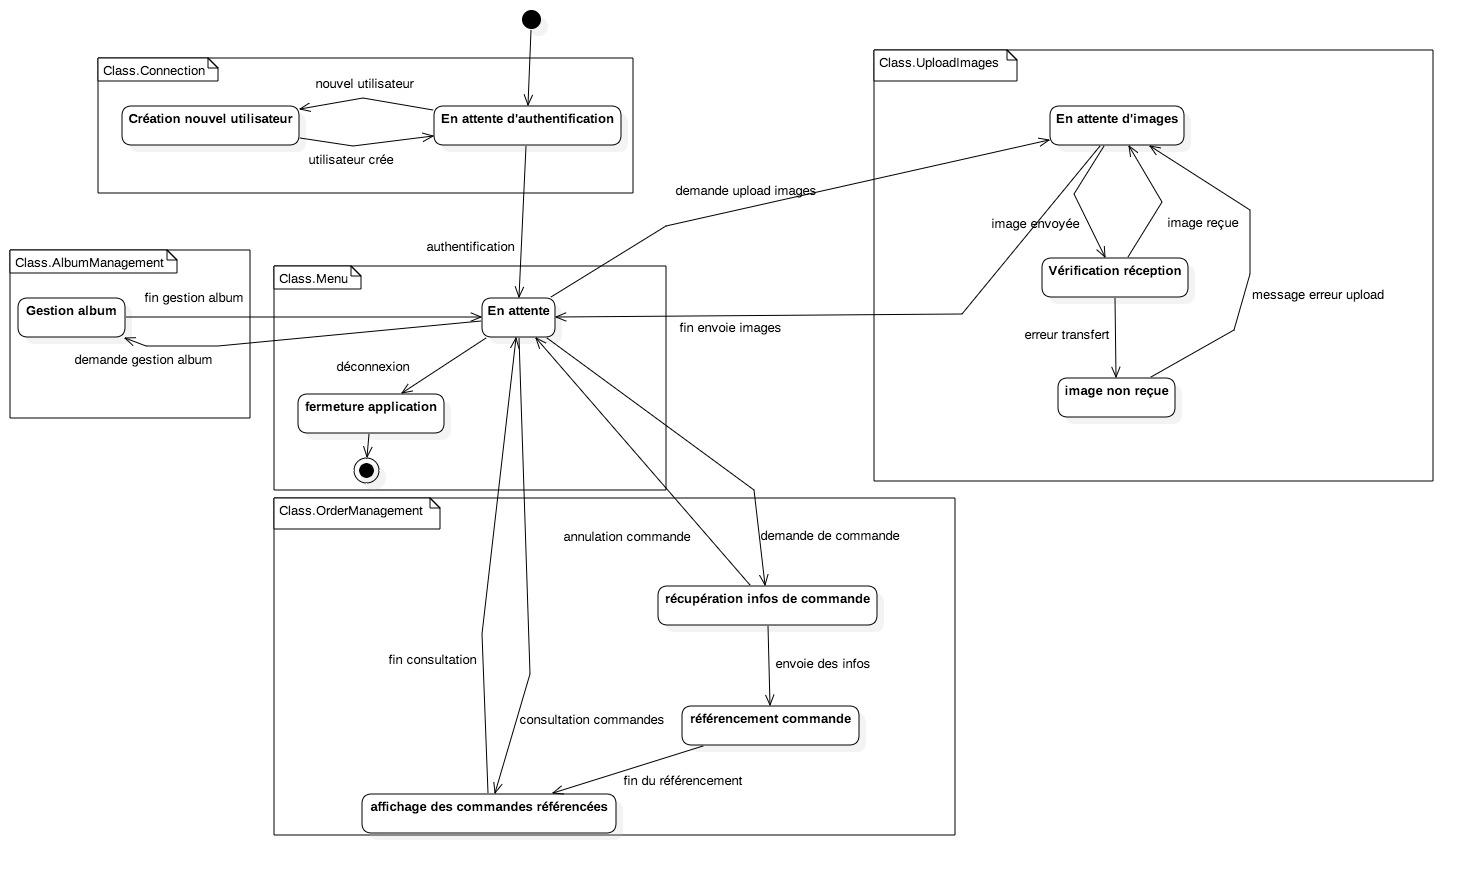
\includegraphics[scale=0.3]{fig2} % Include the image placeholder.png
    \caption{Diagramme d'état du logiciel Esyphoto}
  \end{center}
\end{figure}

Voici notre vision et notre implémentation : \\
\vspace{1\baselineskip}
\begin{itemize}
  \item -- Vue --
\end{itemize}



Une classe View qui possède des méthodes displayX pour les X fonctionnalités
(displayConnection, displayMenu etc)\\
Attributs :\\
- x controlerX; où x est le nombre de fonctionnalités
\vspace{1\baselineskip}
\begin{itemize}
  \item -- Contrôleur --
\end{itemize}


Une classe Controler pour chaque fonctionnalité qui reçoit des notifications
de changement depuis View, grâce à la méthode notifyChangement(). C'est à
partir de cette méthode que les méthode displayX() sont lanceés. Si besoin
elle fait appel aux méthodes de la classe Modèle.\\
Attributs :\\

- Model modèle;\\
- View vue;\\

\vspace{1\baselineskip}
\begin{itemize}
  \item -- Modèle --
\end{itemize}

Une classe Modele qui possède en attribut toutes les classes DAO. Elle
présente des méthodes comme getClientPassword(String) qui permettent de
récupérer des informations dans la base de donnée grâce aux classe DAO.\\
Attributs :\\
- clientDAO, AlbumDAO etc ...
\vspace{1\baselineskip}

Le pattern MVC a été pensé pour respecter au maximum les cloisons entre Model,
View et Controller. Pour cela, nous avons privilégié le schéma de principe
suivant : La partie View, quand elle reçoit une interaction de l’utilisateur
transfère l’information au controller. Ce dernier effectue les tâches et fait
appel au Model avant de transmettre une nouvelle information au View.
Ainsi, mise à part les méthodes display(), la partie View pourrait devenir une
Interface Graphique sans impacter le reste du programme. Dans la même idée le
controller qui ne reçoit et envoi que des String (ou liste de String)
n’impacterait en rien le reste du code avec un changement. Le Model quand
à lui ne transmet des informations que sur demande.\\
\vspace{1\baselineskip}
Note sur le modèle : les seules fonctions qui présentent des affichages
sont à destinations des administrateurs et donc ne sont pas à prendre en
compte dans le pattern.

\begin{figure}[!h]
  \begin{center}
    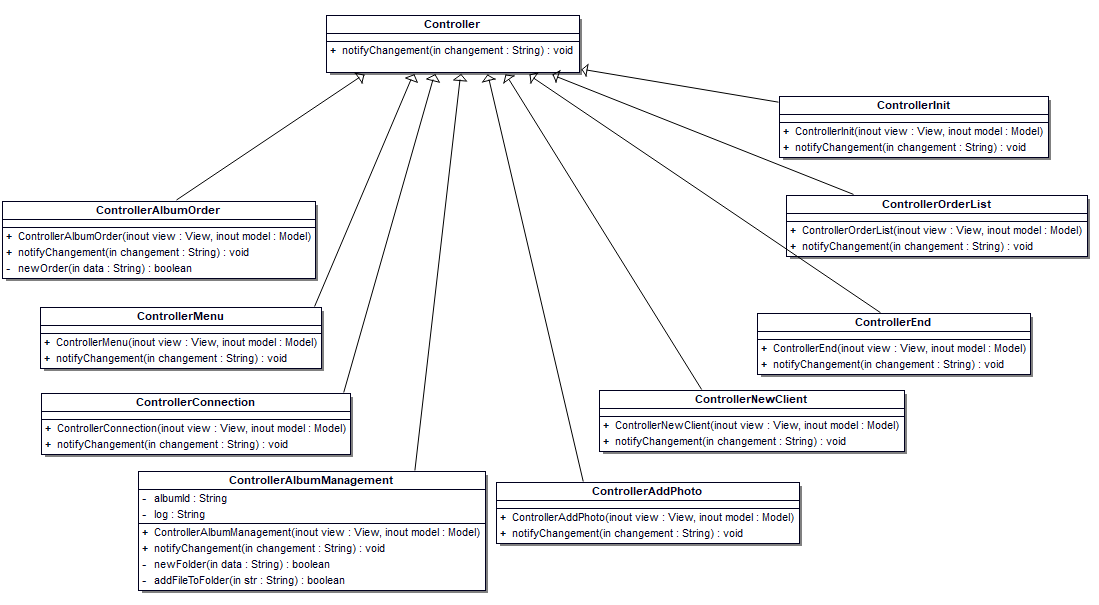
\includegraphics[scale=0.45]{fig6} % Include the image placeholder.png
    \caption{Diagramme du Controller}
  \end{center}
\end{figure}

Ce diagramme représente le fonctionnement détaillé de la partie Controller.
\vspace{1\baselineskip}
\begin{figure}[!h]
  \begin{center}
    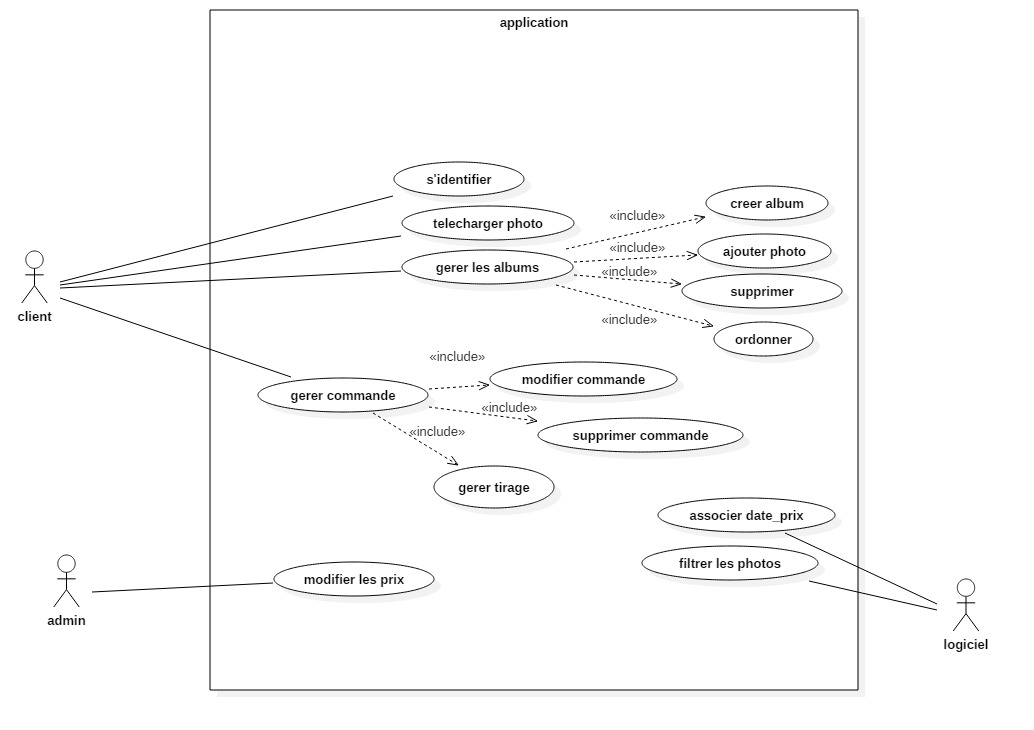
\includegraphics[scale=0.40]{fig7} % Include the image placeholder.png
    \caption{Diagramme de cas d'utilisation}
  \end{center}
\end{figure}

\vspace{1\baselineskip}
\begin{figure}[!h]
  \begin{center}
    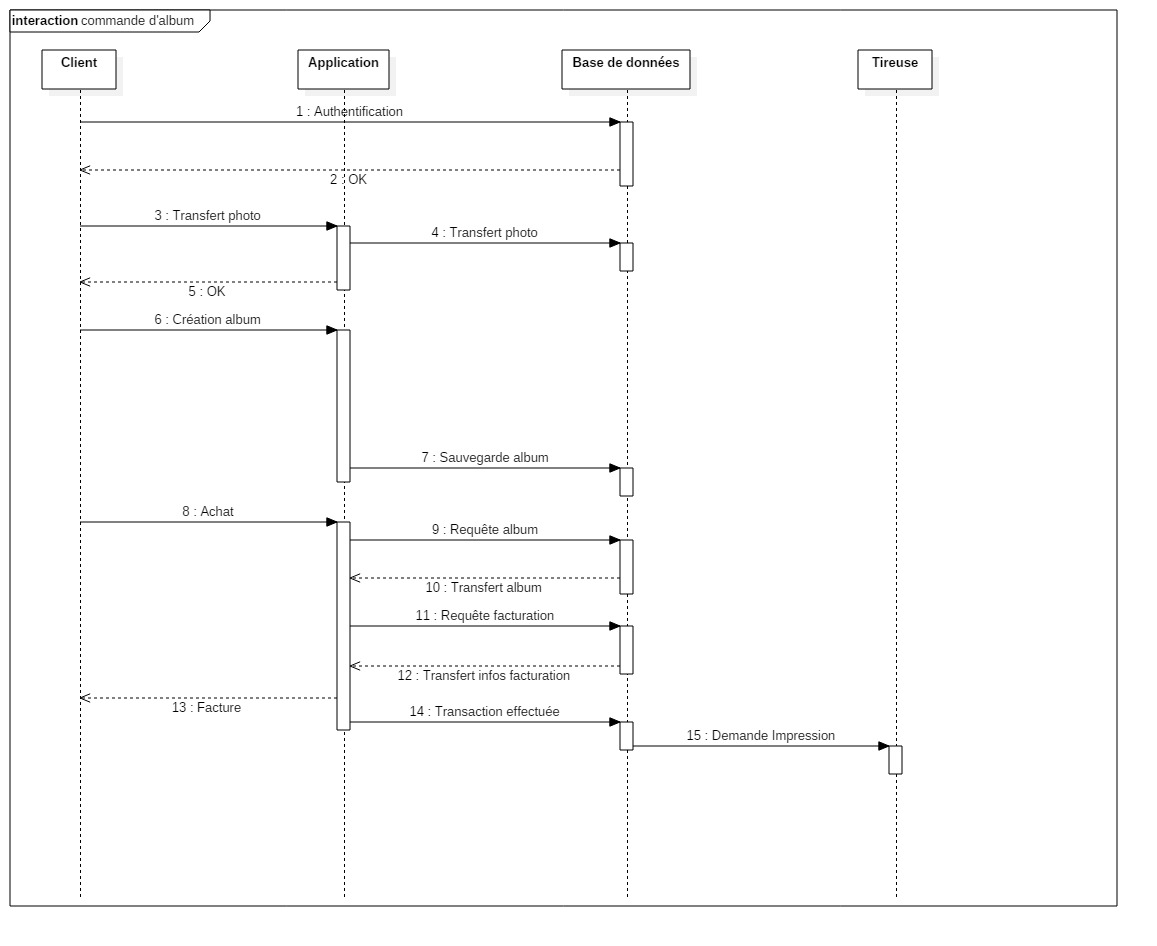
\includegraphics[scale=0.40]{fig8} % Include the image placeholder.png
    \caption{Diagramme de séquence pour la commande d'un album}
  \end{center}
\end{figure}

Le build ANT fourni avec le projet permet de produire 4 exécutables
différents.\\
Exécutables pour utilisateur : \\
\begin{itemize}
  \item CS441_2.jar qui est l'exécutable permettant de lancer le programme
\end{itemize}
Exécutables pour administrateur :\\
\begin{itemize}
  \item deleteTable.jar qui permet d’effacer la table entièrement
  \item initTable.jar qui permet d’initialiser les tables de la base de donnée.
  Obligatoire après avoir effacé la table.
  \item showTable.jar qui permet de rendre compte de l’ensemble des tables
  sur la bases de données.
\end{itemize}


\newpage
\section{Organisation du travail et répartition des tâches}

\begin{figure}[!h]
  \begin{center}
    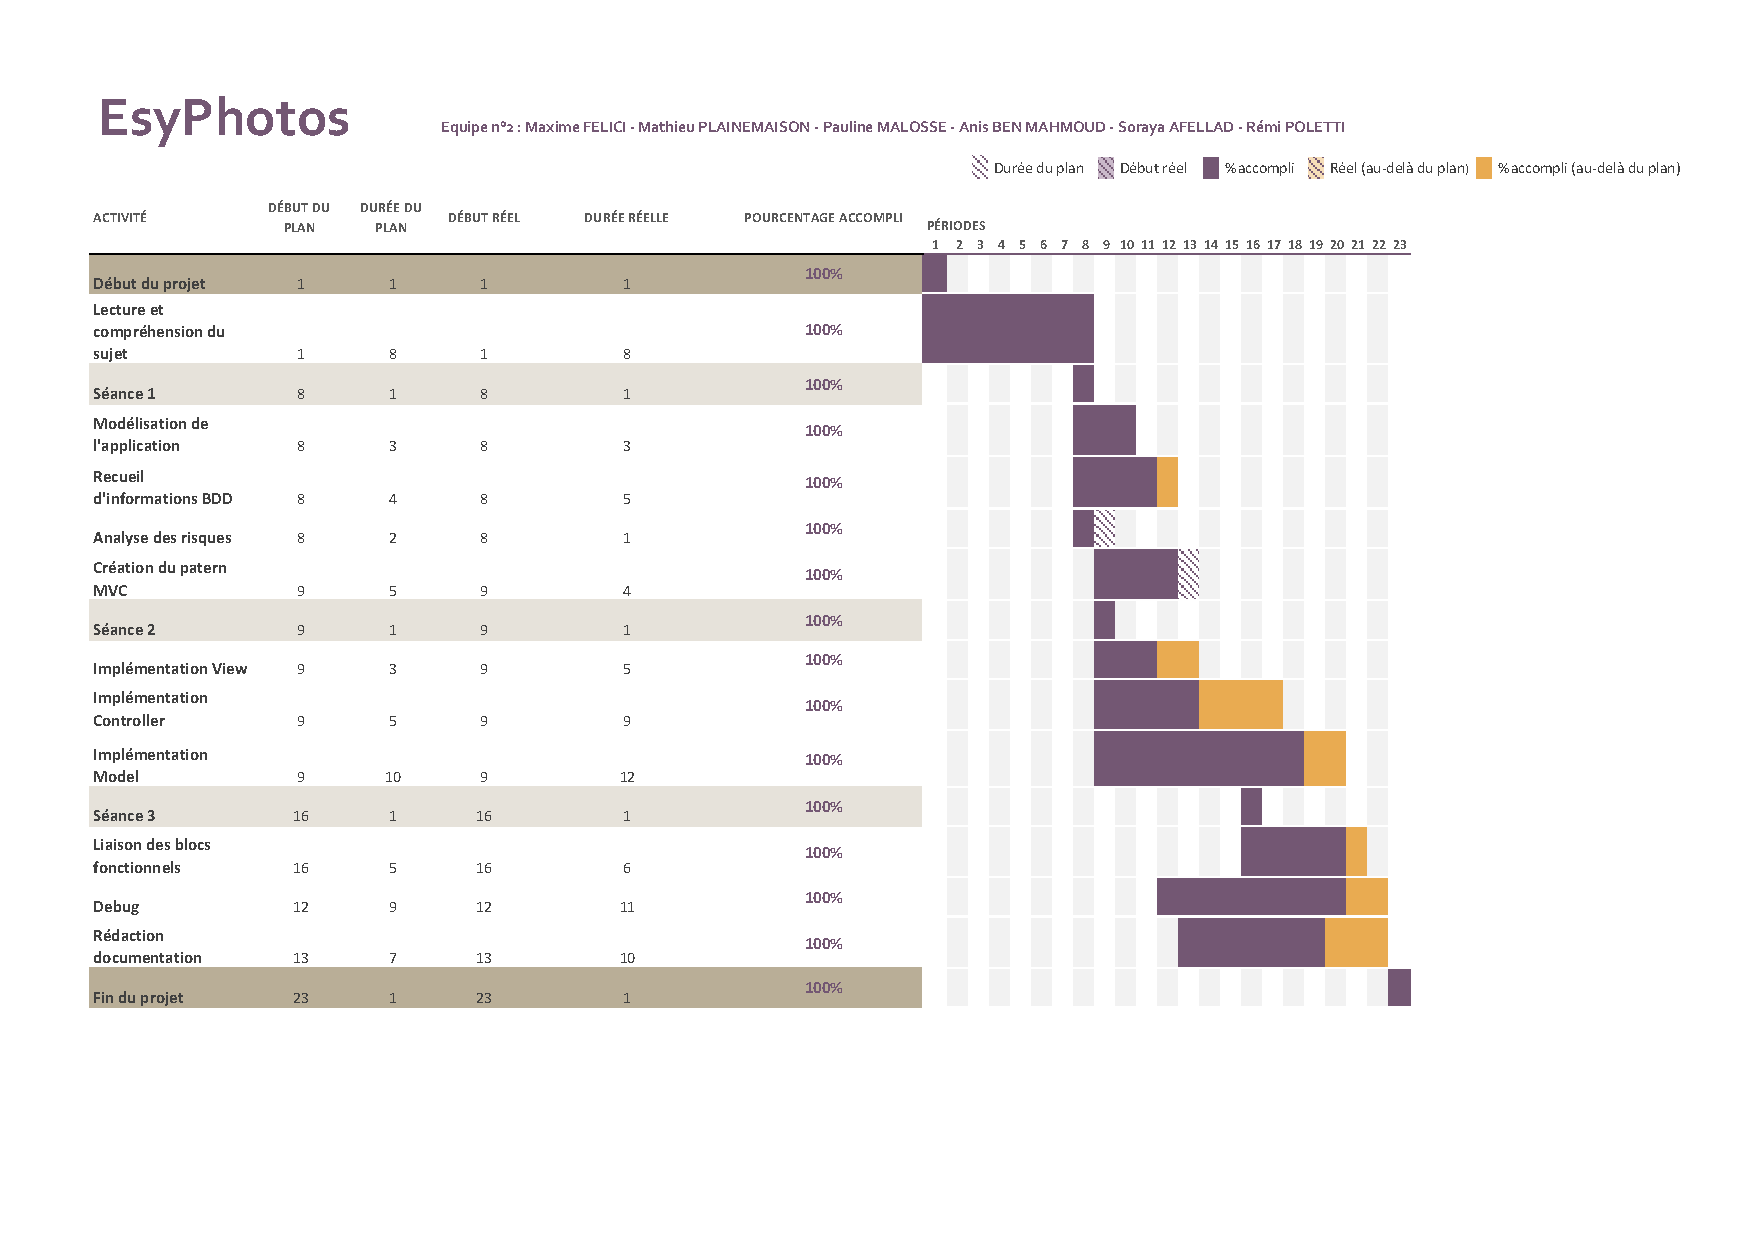
\includegraphics[scale=0.5]{fig4} % Include the image placeholder.png
    \caption{Planning prévisionnel et réel (figure vectorisée, vous pouvez zoomer dessus)}
  \end{center}
\end{figure}

Nous avons réparti les tâches de la manière suivante : \\

\begin{itemize}
  \item Mathieu PLAINEMAISON : Chef de projet, il s'occupe de l'organisation
  générale. Il surveille l'avancement de chacun.
  \item Pauline MALOSSE et Anis BEN MAHMOUD : Ils gèrent l'implémentation
  de la base de donnée.
  \item Rémi POLETTI : Intégration de la partie Controlleur.
  \item Maxime FELICI : Gestion du GIT. Intégration de la partie View.
  Documentation.
  \item Soraya AFELLAD : Conception des diagrammes UML.
\end{itemize}

\newpage
\section{Critique de notre projet}
Rétrospectivement, nous avons remarqué un point faible de notre programme.
En effet, comme les méthodes display() de la classe View appellent toutes
les méthodes notifyChangement() des classes Controller et que ces dernières
appellent les premières, le programme est en réalité une imbrication de
méthodes aux nombre indéterminé. Si cela ne pourrait pas poser de problèmes
au premiers abords, il est facilement compréhensible que cela représente une
instabilité du programme. En effet, lorsque l’utilisateur quitte l’IHM,
l’ensemble des méthodes se termine les unes après les autres ce qui peut
etre source de bugs. Cela impact donc le caractère évolutif de notre travail.
En conséquence, si nous devions refaire cet exercice, nous essayerons de
retravailler le pattern.



\section{Conclusion}
Pour tous les membres de l'équipe, c'était la première fois que nous
travaillons sur un projet avec 5 autres personnes. Cela nous a permis
d'apprendre à correctement utiliser un gestionnaire de versions (Git). Nous
avons dû nous organiser précisemment afin de rendre le travail le plus efficace
possible. Nous avons utilisé le logiciel Slack afin de communiquer plus
facilement. \\
Ce projet nous a permis de manipuler une base de donnée et de créer un
programme complet. Nous avons mit en pratique nos connaissances du cours
de Génie Logiciel (UML, Cycle de vie, Base de données), mais aussi de nos cours
précédents de Java.





%---------------------------------
\end{flushleft}
%---------------------------------
\end{document}
